\documentclass[11pt]{article}
\usepackage[letterpaper,margin=1in]{geometry}
\usepackage{amsmath,amssymb,amsthm}
\usepackage{tikz}
\usetikzlibrary{arrows,shapes,positioning}

\title{Formal Causal Framework for Scoring Bias}
\author{}

\begin{document}
\maketitle

\section{Formal Definitions}

\begin{definition}[Scoring Bias]
Let $f_\theta(p, r)$ be the score assigned by model $\mathcal{M}_\theta$ to response $r$ given prompt $p = (i, s)$ where $i$ is the instruction and $s$ is the scoring instruction. A \emph{scoring bias} exists if:
\[
\mathbb{E}[f_\theta(p, r)] \neq \mathbb{E}[f_\theta(p', r)]
\]
for some $p'$ that is semantically equivalent to $p$ (same scoring task) but differs in a non-diagnostic feature (scale direction, label format, exemplar presence).
\end{definition}

\begin{definition}[Differential Effect]
Let $\theta_B$ and $\theta_I$ be base and instruct parameters. The differential effect $\delta$ for bias probe $b$ is:
\[
\delta_b = |\mathbb{E}[f_{\theta_I}(p_b, r)] - \mathbb{E}[f_{\theta_I}(p_b', r)]| - |\mathbb{E}[f_{\theta_B}(p_b, r)] - \mathbb{E}[f_{\theta_B}(p_b', r)]|
\]
where $p_b, p_b'$ are the control and biased prompts for probe $b$.
$\delta_b < 0$ means instruction tuning reduces bias for probe $b$.
\end{definition}

\section{Causal Identification Assumptions}

For the claim ``instruction tuning causes the differential effect'' to be valid:

\begin{enumerate}
    \item \textbf{Consistency:} $f_{\theta_I}(p, r) = f_{\theta_I}(p, r)$ holds as defined.
    \item \textbf{Positivity:} For each base model, an instruct-tuned version exists.
    \item \textbf{SUTVA:} No interference between models. Stable unit treatment value.
    \item \textbf{Comparability:} Base and instruct variants are identical except for the training stage.
\end{enumerate}

Assumption 4 is partially violated: instruct variants are typically larger (additional layers, LoRA adapters) or trained on different schedules. We mitigate by comparing only within-family.

\section{Causal DAG}

\[
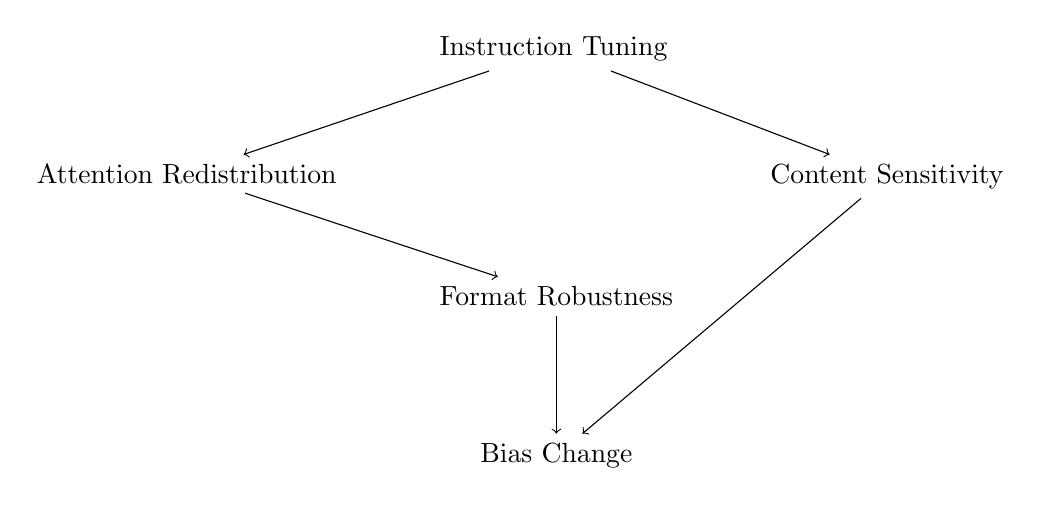
\begin{tikzpicture}[node distance=1.5cm, auto]
\node (T) {Instruction Tuning};
\node (A) [below left=of T] {Attention Redistribution};
\node (F) [below right=of A] {Format Robustness};
\node (C) [below right=of T] {Content Sensitivity};
\node (B) [below=of F] {Bias Change};
\draw[->] (T) to (A);
\draw[->] (A) to (F);
\draw[->] (T) to (C);
\draw[->] (F) to (B);
\draw[->] (C) to (B);
\end{tikzpicture}
\]

\section{Measurement Invariance}

For valid cross-model comparison, the bias score must satisfy:
\[
\text{Cov}(f_{\theta_1}(p, r), \text{bias}_1) = \text{Cov}(f_{\theta_2}(p, r), \text{bias}_2)
\]
where $\text{bias}_i$ is the latent bias propensity of model $i$. We assume weak invariance.

\section{Identification Strategy}

Our strategy is difference-in-differences: for each model family, we compute the change in bias from base to instruct. The average treatment effect on the treated (ATT) is:
\[
\tau = \mathbb{E}[\delta | \theta = \theta_I] - \mathbb{E}[\delta | \theta = \theta_B]
\]

This removes time-invariant model family characteristics. Remaining threats:
\begin{enumerate}
    \item Differential training data quality between base and instruct.
    \item Different model size for base vs instruct.
    \item Platform differences (local vs API inference).
\end{enumerate}

\end{document}
